\scanpage{19}

\figure{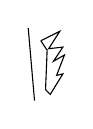
\begin{tikzpicture}[x=.4cm,y=.4cm]\draw (0,0)--(-.2,2.3);\draw (.2,1.9)--(.8,2.2)--(.45,1.65)--(.9,1.7)--(.6,1.25)--(.95,1.45)--(.7,.8)--(.9,.85)--(.5,.2)--(.35,.35)--(.4,1.6)--(.2,1.9);\end{tikzpicture}}
$b$

\uuline{$j$ et $j-1$ \unsure{unité}}

Cas $A$ \unsure{local} \uline{normal}
\[
\left\{\begin{array}{ll}
j\text{ une unité, pas }j-1,\ \unsure{(\text{par idéal})}&(1-j^{-1})^2\in A^6\unsure{A^*}\\
j-1\text{ une unité, }j\text{ pas}\ \unsure{(\text{par idéal})}&\left(\dfrac{j}{j-1}\right)^3\in A^6A^*
\end{array}\right.
\]

\figure{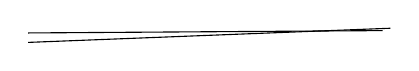
\begin{tikzpicture}\draw (0,0)--(4.5,.03);\draw (0,-.12)--(4.6,.06);\end{tikzpicture}}
\margin{\uline{à vérifier} \uline{\unsure{géométriquement}}}
\diagram{\begin{tikzcd}[column sep=large]
\text{Ext. Kummérienne de gr }\mathbb Z/3 \arrow[r,leftrightarrow]& j\equiv1
\end{tikzcd}}
\[
b^3=0,\quad c\text{ inversible}\quad //
\]
Si \deleted{\unsure{a}} $A$ \unsure{ss élémts nilpotts}, alors l'invariant
\[
c\in A^*/A^{*(3)}.
\]
\diagram{\begin{tikzcd}[column sep=large]
\text{Ext. Kummérienne de gr }\unsure{Z|\mathbb Z}/2 \arrow[r,leftrightarrow]&j\equiv0
\end{tikzcd}}
\[
c^2=0,\quad b\text{ inversible}\quad //
\]
Si $A$ \unsure{ss élémts nilpotts} alors l'invariant est
\[
b\in A^*/A^{*(2)}.
\]
\hrulefill

\hfill $1-$

\figure{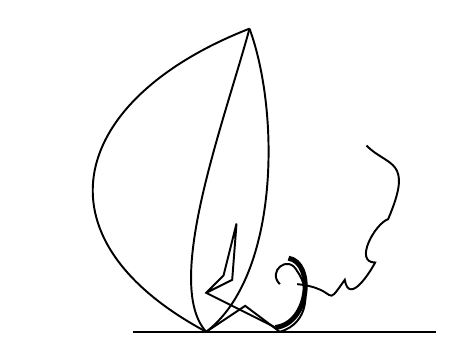
\begin{tikzpicture}[x=.55cm,y=.55cm,line width=.7pt]
\draw (-.6,0)--(6.4,0);
\draw (2.1,7) .. controls (-2,5.4) and (-3,2.2) .. (1.1,0) .. controls (2.8,1.3) and (2.8,5.1) .. (2.1,7);
\draw (2.1,7) .. controls (1.5,4.8) and (.1,1.1) .. (1.1,0);
\draw (1.1,0)--(2,.6)--(2.8,0) .. controls (3.5,.2) and (3.5,1) .. (3.2,1.4) .. controls (3,1.8) and (2.5,1.4) .. (2.8,1.1);
\draw[line width=1.8pt] (2.7,.1) .. controls (3.5,.2) and (3.6,1.6) .. (3,1.7);
\draw (1.1,.9)--(1.7,1.2)--(1.8,2.5)--(1.5,1.3)--(1.1,.9)--(2.7,.1);
\draw (3.2,1.1) .. controls (4.2,1) and (3.8,.5) .. (4.3,1.2) .. controls (4.4,.6) and (4.9,1.4) .. (5,1.6) .. controls (4.5,1.6) and (5,2.5) .. (5.3,2.6) .. controls (5.9,4) and (5.3,3.8) .. (4.8,4.3);
\end{tikzpicture}}
\[
\deleted{\unsure{j}}\quad\left(\frac{t}{t-1}\right)^3\in O^6O^*\qquad\uline{\unsure{\text{module}\ p|\text{unité}\ pr}}
\]
\[
\left(\frac{t-1}{t}\right)^2\in O^6O^*\qquad\text{``}\qquad
\sqrt[6]{\frac{t\deleted{\unsure{t}}}{t-1}}
\]
\hrulefill

\figure{
\begin{tikzpicture}[x=.7cm,y=.7cm]\draw[line width=3pt] (0,0) circle (.42);\end{tikzpicture}}
\[
\sqrt[2]{\frac{t}{t-1}}\qquad\sqrt[3]{\frac{t-1}{t}}\qquad \tfrac12\qquad\tfrac13
\]
\figure{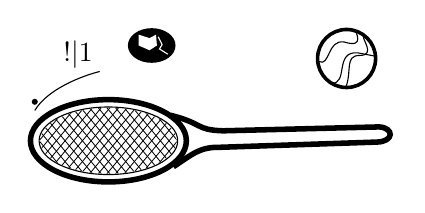
\begin{tikzpicture}[x=.55cm,y=.55cm]
\node at (-.7,2.2) {$\unsure{!|1}$};
\fill (1,2.4) ellipse (.55 and .4);
\fill[white] (.7,2.65)--(.95,2.57)--(1.1,2.65)--(1.12,2.4)--(.95,2.29)--(.7,2.4)--cycle;
\draw[white] (1.15,2.6)--(1.24,2.42)--(1.18,2.32)--(1.37,2.2);
\draw[line width=1.3pt] (5.5,2.1) circle (.67);
\draw (4.86,2.03) .. controls (5.12,1.9) and (5.05,2.55) .. (5.45,2.48) .. controls (5.95,2.32) and (5.68,2.75) .. (5.72,2.73);
\draw (5.15,1.53) .. controls (5.55,1.5) and (5.21,2.28) .. (5.76,2.23)--(6.13,2.16);
\draw (5.48,1.43) .. controls (5.63,1.81) and (5.45,2.17) .. (5.8,2.17) .. controls (6.2,2.17) and (5.82,2.58) .. (5.9,2.62);
\fill (-1.7,1.1) circle (.07);
\draw[line width=2pt] (0,.2) ellipse (1.8 and .95);
\draw (0,.2) ellipse (1.6 and .78);
\begin{scope}\clip (0,.2) ellipse (1.58 and .76);
\foreach \k in {-3,-2.8,...,3}{\draw[line width=.3pt] (\k,-1)--(\k+2,1.4);\draw[line width=.3pt] (\k,-1)--(\k-2,1.4);}\end{scope}
\draw[line width=2pt] (1.43,.79) .. controls (2.2,.6) and (2,.45) .. (2.65,.43)--(6.25,.52) .. controls (6.6,.5) and (6.6,.18) .. (6.2,.17)--(2.6,.05) .. controls (2.1,.06) and (1.96,-.1) .. (1.5,-.4);
\draw (-1.7,.9) .. controls (-1.4,1.4) and (-.6,1.7) .. (-.2,1.8);
\end{tikzpicture}}
\[
\lambda^{3/6}\cdot\lambda^{\unsure{-2/6}}=\lambda^{1/6}\qquad
\frac{-27c^{\unsure{2}}}{b^3-27c^2}=j
\]
\figure{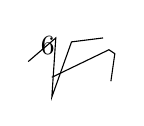
\begin{tikzpicture}[x=.5cm,y=.5cm]\node at (0,1) {$6$};\draw (-.5,.6)--(.2,1.2)--(.1,-.3)--(.6,1.1)--(1.4,1.2);\draw (.1,.2)--(1.55,.9)--(1.7,.8)--(1.6,.1);\end{tikzpicture}}
\[
s^6=\frac{t}{t-1}\qquad \frac{b^3}{c^2}=j\qquad 27c^2(j-1)=b^3j
\]
\diagram{\begin{array}{ccc}L&L^2&L^3\\&b&c\end{array}}
\[
b^{\deleted{\unsure{3}}}=27\frac{j-1}{j}\qquad
\boxed{\frac{b^3}{c^2}=27\frac{j-1}{j}}
\]
\figure{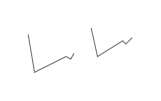
\begin{tikzpicture}[x=.4cm,y=.4cm]\draw[gray] (0,1.2)--(.2,0)--(1.2,.5)--(1.35,.42)--(1.45,.6);\draw[gray] (2,1.4)--(2.2,.5)--(3,1)--(3.1,.9)--(3.3,1.1);\end{tikzpicture}}
\figure{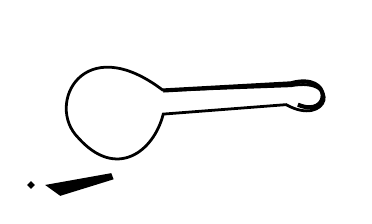
\begin{tikzpicture}[x=.6cm,y=.6cm,line width=1pt]\draw (0,0) .. controls (-1.7,1.3) and (-2.5,-.3) .. (-1.8,-1) .. controls (-1,-1.9) and (-.2,-1.3) .. (0,-.5)--(2.6,-.3) .. controls (3.5,-.8) and (3.8,.3) .. (2.7,.1)--(0,0);\draw[line width=1.5pt] (0,0)--(2.7,.15) .. controls (3.6,.4) and (3.55,-.6) .. (2.85,-.3);\fill (-2.5,-2)--(-1.1,-1.75)--(-1.05,-1.88)--(-2.18,-2.23)--cycle;\draw (-2.8,-2) circle (.04);\end{tikzpicture}}
\[
c=27\frac{j-1}{j}
\]
\deleted{\unsure{Hom}($\unsure{\widetilde E}$,)}
\[
f_*(\widetilde E)
\]
\diagram{\begin{tikzcd}
&\unsure{\underline{\mathrm H}|\underline{\mathrm{Hom}}}_{\unsure{O|0}}(E,\unsure{\underline O|\underline U})\\
\unsure{\underline{\mathrm H}|\underline{\mathrm{Hom}}}_{\underline A}(\widetilde E,\underline A)\times&\unsure{\underline{\mathrm H}|\underline{\mathrm{Hom}}}_{\underline O}(\underline A,\underline O)\arrow[u]
\end{tikzcd}}
\[
\boxed{x^3+27\frac{j-1}{j}(x+1)=0}
\]
\mspage{18}
